\documentclass[11pt]{amsart}

\usepackage{amsthm, amssymb,amsmath, listings}
\usepackage{enumitem}
\usepackage{graphicx}
\usepackage{faktor}
\usepackage[utf8]{inputenc}
\usepackage[english]{babel}
\usepackage{fancyhdr}


\theoremstyle{definition}  % Heading is bold, text is roman
\newtheorem{theorem}{Theorem}
\newtheorem{definition}{Definition}
\newtheorem{example}{Example}
\oddsidemargin 0pt
\evensidemargin 0pt
\marginparwidth 0pt
\marginparsep 10pt
\topmargin 0pt
\headsep 20pt
\textheight 9in
\textwidth 6.5in
%New command wasteland
\newcommand{\ojo}[1]{{\sffamily\bfseries\boldmath[#1]}}

\newcommand{\seq}[2]{#1_1#2_1,...,#1_n#2_n}
\newcommand{\sumseq}[2]{#1_1#2_1+...+#1_n#2_n}
\newcommand{\inpr}[1]{\langle #1 \rangle}
\newcommand{\norm}[1]{\lvert #1 \rvert}
\newcommand{\Hilb}{\mathcal{H}}
\newcommand{\Kilb}{\mathcal{K}}
\newcommand{\Z}{\mathbb{Z}}
\newcommand{\N}{\mathbb{N}}
\newcommand{\Q}{\mathbb{Q}}
\newcommand{\R}{\mathbb{R}}
\newcommand{\C}{\mathbb{C}}
\newcommand{\nullspace}{\mathrm{null}}
\newcommand{\rank}{\mathrm{rank}} 
\newcommand{\compconj}[1]{ \overline{#1}}

%Setting commands
\newcommand{\name}{Juniper Overbeck}
\newcommand{\ttle}{}


%FancyHF stuff, capitalization brutalized.
\pagestyle{fancy}
\fancyhf{}
\lhead{\ttle}
\rhead{\name}
\cfoot{}
\fancypagestyle{plain}{ %
	\fancyhf{}
	\renewcommand{\headrule}{} % remove lines as well
	\cfoot{}
}


\renewcommand\headrule{
	\begin{minipage}{1\textwidth}
        \begin{center}
		\hrule width \hsize \kern 1mm \hrule width \hsize height 2pt
        \end{center}
	\end{minipage}
}

\begin{document}

\begin{flushleft}
	\Large\textbf{\ttle}\\
	\small{\textbf{\name}}\\
\end{flushleft}
\noindent\makebox[\linewidth]{\rule{\textwidth}{0.4pt}}\\[-8px]
\noindent\makebox[\linewidth]{\rule{\textwidth}{1pt}}\\[9px]
\section{Syllabus Review}
    \begin{enumerate}
        \item Pictures + Computer are ok so long as they're used for note taking.
        \item Expect for the tests to be at ends of the first third of the class, and the second third of the class.
        \item Theoretically this is a graduate course, and will be switched to 852, rather than remaining as 452.
    \end{enumerate}


\section{Day 1}
\subsection{Syllabus Junk}
    \begin{itemize}
        \item Pictures + Computer are ok so long as they're used for note taking.
        \item Expect for the tests to be at ends of the first third of the class, and the second third of the class.
        \item Theoretically this is a graduate course, and will be switched to 852, rather than remaining as 452.
    \end{itemize}
\subsection{The idea of algebraic topology}
    \begin{itemize}
        \item Given topological spaces $X$ and $Y$, how can we prove that $X$ and $Y$ are or aren't homeomorphic.
        \item To prove $X\cong Y$, we simply exhibit a homeomorphism.\\
            E.g. $(-1,1) \cong \R$, using $f(x) = \frac{x}{1-x^2}$\\
            E.g. $\square \cong \circ$
        \item To prove $X\ncong Y$, we'd find a topological invariant, (connected, compact, Hausdorff,\ldots), that only one has.\\
            E.g. $(0,1) \ncong [0,1]$, here, the closed interval is compact, and the open interval is not.\\
            E.g. $(0,1) \ncong [0,1)$, because,\\
            \begin{align*}
                [0,1)\setminus \{0\} = (0,1) \text{ which is connected, but}\\
                (0,1)\setminus \{\text{any point}\} \text{ is disconnected}\\
            \end{align*}
            Note, with the following exercise, If $X\cong Y$ via a homeomorphism, $\psi : X\rightarrow Y$,
            then $X\setminus\{p\}\cong Y\setminus \{\psi(p)\}$
        \item Show the following. \\
            \begin{align*}
                \R \ncong \R^2\\
            \end{align*}
            Here, we note that $\R \setminus \{0\}$ is disconnected.\\
            Suppose towards contradiction that $\R \cong\R^2$, call the homeomorphism $\phi:\R\rightarrow \R^2$, because
            $\R\setminus \{0\}$, the excercise implies that $\R\setminus \{0\}\cong \R^2\{\phi(0)\}$, and therefore
            $\R^2\setminus\{\phi(0)\}$ is disconnected, but that's just wrong, because $\R^2$ without a single point
            is still connected, rigorously showing this should be done through working with path connectedness. Therefore
            these are not homeomorphic.
            \begin{align*}
                \R^2 \ncong \R^3\\
            \end{align*}
            This was a trick question, we don't actually have any topological properties that we can rely on. If we were
            to attempt to remove a line from $\R^2$, we don't have enough information about what the line is homeomorphic to
            in $\R^3$, which is the major stumbling block.
        \item\underline{The Fundamental Group}
        \item The fundamental group is a waay to associate a topological space $X$ to a group $\pi_1(X)$ so that
            $X\cong Y \Rightarrow \pi_1(X)\cong\pi_2(Y)$. 
        \item We'll be able to use this to prove spaces aren't homeomorphic.\\
            \underline{Ex:} In this course we'l learn the following.
            \begin{align*}
                \pi_1(\R^2\setminus\{(0,0)\})=\Z\\
                \pi_2(\R^3\setminus\{\text{any point}\})=\{1\}\\
                \pi_1(\R^2\setminus\{(0,0)\})\ncong \pi_2(\R^3\setminus\{\text{any point}\})\\
                \R^2\ncong\R^3\\
            \end{align*}
            Using this, we can show that these things are not homeomorphic, which is why we do algebraic topology.
            More powerful tools allow for more results.
        \item Note: It's not true that $\pi_1(X)\cong \pi_2(Y)\Rightarrow X\cong Y$\\
            More generally, algebraic topology is about associating the topological space $X$ 
            with the algebraic object $A(X)$, in such a way that $X\cong Y \Rightarrow A(X)\cong A(Y)$\\
            There's a spectrum though.
            \begin{enumerate}
                \item Easy to compute and says nothing, $A(x)$ is the same for all of $X$
                \item Hard to compute, but says everything, $A(X)\cong A(Y) \iff X\cong Y$
            \end{enumerate}
    \end{itemize}

\section{Day 2}
\subsection{The Fundamental Group}
    \begin{itemize}
        \item Idea: $\pi_1(X)=\faktor{\{\text{``loops'' in X}\}}{\sim}$, where $L_1 \equiv L_2$ if $L_1$ can be ``deformed'' inside $X$
            into $L_2$
        \item \underline{Ex:} Last time it was claimed that $\pi_1(\R^2\setminus \{(0,0)\})=\Z$.
        \item\underline{Paths and Homotopies}
        \item Let $X$ be a topological space.
    \end{itemize}
        \begin{definition}
            A \underline{path} in $X$ is a continuous map $f:I \rightarrow X$, where $I=[0,1]\subseteq \R$ (with the
            subspace topology from the Euclidean topology on $\R$.\\
            If $f(0)=p$ and $f(1)=q$, we say $f$ is a path \underline{from $p$ to $q$}.
        \end{definition}
    \begin{itemize}
        \item \underline{Ex:}
            \begin{align*}
                X&=\R^2\\
                f: I &\rightarrow\R^2\\
                f(t)&=(1-2t,0)\\
            \end{align*}
            $f$ is a path in $\R^2$ from $(1,0)$ to $(-1,0)$.
        \item Another path in $\R^2$ from $(1,0)$ to $(-1,0)$ is,
            \begin{align*}
                g: I &\rightarrow \R^2\\
                g(t)&=(\cos(\pi t),\sin(\pi t))\\
            \end{align*}
        \item To make precise, ``Deforming'' one path into another:\\
            \begin{minipage}[c]{\linewidth}
                \begin{center}
                    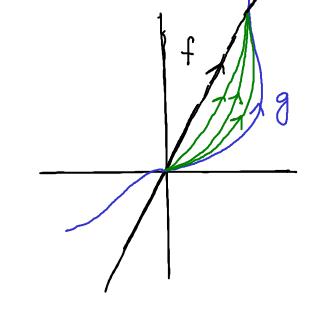
\includegraphics[]{images/homotopy_class_2.png}
                \end{center}
            \end{minipage}\\
    \end{itemize}
        \begin{definition}
            Let $f$ and $g$ be paths in $X$ from $p$ to $q$. A \underline{path homotopy} from $f$ to $g$ is a continuous function,
            \begin{align*}
                H: I\times I \rightarrow X\
            \end{align*}
            (note that elements of $I\times I$ resemble, $(s,t)$)
            Such that,
            \begin{align*}
                H(s,0)&=f(s),\ \forall s\\
                H(s,1)&=g(s),\ \forall s\\
                H(0,t)&=p,\ \forall s\\
                H(1,t)&=q,\ \forall s\\
            \end{align*}
        \end{definition}
    \begin{itemize}
            To make sense of this, define, $\forall t$,
            \begin{align*}
                h_t: I&\rightarrow X\\
                h_t(s)&=H(s,t)\\
            \end{align*}
            Then, $\forall t$,
            \begin{align*}
                h_t= \text{ path in $X$ from $p$ to $q$ }\\
            \end{align*}\\
            \begin{minipage}[c]{\linewidth}
                \begin{center}
                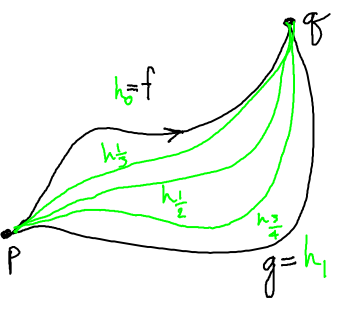
\includegraphics[]{images/homotopy_class.png}
                \end{center}
            \end{minipage}
            This is continuous because $H$ is continuous, and it goes from $p$ to $q$, because $h_t(0)=H(0,t)=p$ and $h_t(1)=H(1,t)=q$.
            $h_0(s)=f$ because $h_0(s)=H(s,0)=f(s),\ \forall s$\\
            and $h_1(s)=g$ because $h_1(s)=H(s,1)=g(s),\ \forall s$\\
    \end{itemize}
    \begin{definition} If $\exists$ a path homotopy from $f$ to $g$, we say $f$ and $g$ are \underline{path-homotopic}, and $f\cong g$\\
        \underline{Ex:} $X=\R^2$, Let,
        \begin{align*}
            f(s)=(\cos(\pi s), \sin(\pi s))\\
            f(s)=(\cos(\pi s), 2\sin(\pi s))\\
        \end{align*}
        Both are paths in $\R^2$ from $(1,0)$ to $(-1,0)$.\\
        Then,
        \begin{align*}
            H: I\times I &\rightarrow \R^2\\
            H(s,t)&=(\cos(\pi s), (t+1)*\sin(\pi s))\\
        \end{align*}
        $H$ is a path homotopy from $f$ to $g$, because,
        \begin{align*}
            H(s,0)&=(\cos(\pi s), \sin(\pi s))=f(s)\\
            H(s,1)&=(\cos(\pi s), 2\sin(\pi s))=g(s)\\
            H(0,t)&=(\cos(0), (t+1)\sin(0))=(1,0)\forall t\\
            H(1,t)&=(\cos(\pi), (t+1)\sin(\pi))=(-1,0)\forall t\\
        \end{align*}
    \end{definition}
    \begin{itemize}
        \item \underline{Question:} Find a path homotopy from $\R^2$ from $f(s)=(s,s)$, and $g(s)=(s,s^2)$\\
            Answer(June): $H(s,t)=(s,s^{t+1})$\\
            (see the notebook, there's a solution there. Keep in mind that you want to try to find $p$ and $q$ first, before you do anything else)\\
            Answer(Dr. Clader): General Trick In $\R^2$ let $f$ and $g$ be any two paths from $p$ to $q$, then the
            \underline{straight line homotopy} is as follows,
            \begin{align*}
                H: &I \times I \rightarrow \R^2\\
                H(s,t)&=(1-t)*f(s)+t*g(s)\\
            \end{align*}
            Note that this resembles the stuff you've seen in optimization and advanced linear algebra. This is a pretty powerful tool,
            remember and fear it.
        \item \underline{Ex:} In the question above, $H(s, t)=(s, (1-t)s+ts^2)$
    \end{itemize}

\subsection{Day 3}
    \begin{enumerate}
        \item\underline{Products of Paths}
        \item \underline{Last time:} If $f$ and $g$ are any two paths in $\R^2$ from $p$ to $q$, then $f\cong_{p}q$.
        \item \underline{By contrast:} In, $S'=\{(x,y)\in \R^2| x^2+y^2=1\}$ if
            \begin{align*}
                f(s)&=(\cos(\pi s), \sin(\pi s))\\
                g(s)&=(\cos(\pi s), -\sin(\pi s))\\
            \end{align*}
            Then $f\ncong_{p}g$. (We'll prove this carefully later).
        \item \underline{Fact: (HW)} $\cong_{p}$ is an equivalence relation on the set $\{$paths in $X$ from $x$ to $y\}$
            Thus we can consider the set,
            \begin{align*}
                \faktor{\{ \text{paths in $X$ from $x$ to $y$}\}}{\cong_{p}}\\
                =\{\text{path-homotopy classes of paths in $X$ from $x$ to $y$}\}\ni [f]\\
            \end{align*}
            E.g. in the $S'$ example above, $[f]\neq[g]$
        \item \underline{Def: } Let the following be so,
            \begin{align*}
                X &=\ \text{topological space}\\
                f &=\ \text{path in $X$ from $x$ to $y$}\\
                g &=\ \text{path in $X$ from $y$ to $z$}\\
            \end{align*}\\
            \begin{minipage}[c]{\linewidth}
                \begin{center}
                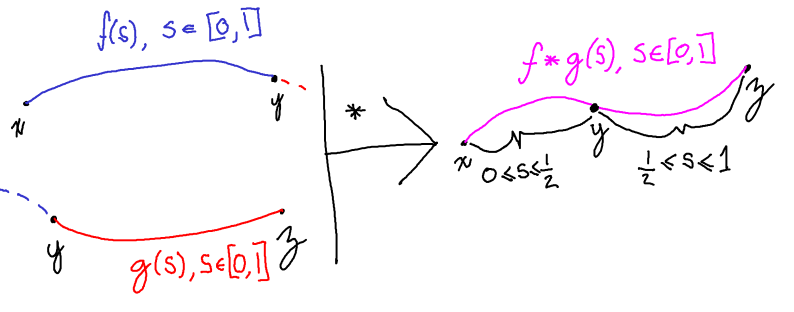
\includegraphics[width=\linewidth]{images/concatenation.png}
                \end{center}
            \end{minipage}
            Then the \underline{concatenation} of $f$ and $g$ is the path $f*g$ from $x$ to $z$ given by,
            \begin{align*}
                f*g: &I \rightarrow X\\
                (f*g)(s)&=\begin{cases}
                    f(2s) & \text{if}\ 0\leq s \leq \frac{1}{2}\\
                    g(2s) & \text{if}\ \frac{1}{2}\leq s \leq 1\\
                \end{cases}\\
            \end{align*}
        \item Why is $f*g$ continuous?\\
        \newpage
        \item \underline{Gluing Lemma:} Let the following be so,
            \begin{align*}
                X &= \text{topological space}\\
                A,B \subseteq X,\ &\text{closed subsets such that } X=A\cup B\\
                Y &= \text{topological space}\\
            \end{align*}\\
                \begin{minipage}[c]{\linewidth}
                    \begin{center}
                    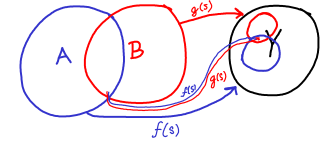
\includegraphics[]{images/gluing_lemma_2.png}
                    \end{center}
                \end{minipage}
            Let the following continuous functions be defined,
            \begin{align*}
                f&: A \rightarrow Y\\
                g&: B \rightarrow Y\\
            \end{align*}
            such that $f(x)=g(x)\ \forall x \in A\cap B$.\\
                        \begin{minipage}[c]{\linewidth}
                            \begin{center}
                            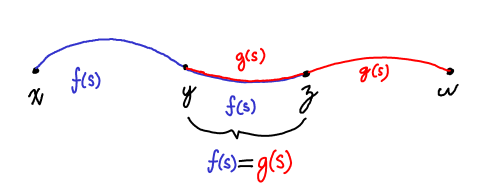
\includegraphics[]{images/gluing_lemma.png}
                            \end{center}
                        \end{minipage}\\ 
                    Then the function,\\
            \begin{align*}
                h: X\rightarrow Y\\
                h(x)=\begin{cases}
                    f(x) & \text{if } x\in A\\
                    g(x) & \text{if } x\in B\\
                \end{cases}\\
            \end{align*}
            is continuous. The proof is left as an exercise to the reader. Thanks. (Homework Problem 1)\\
            \underline{Note:} Applying the gluing lemma to $I = [0,\frac{1}{2}]\cup [\frac{1}{2}, 1]$ shows
            that $f*g$ is continuous.
        \item \underline{Question:} Let the following be so,
            \begin{align*}
                X &= \R^2\\
                f(s)&=(s-1,s)\\
                g(s)&=(s,s+1)\\
            \end{align*}
            What is $f*g$? Draw a picture.
        \item \underline{Answer:} 
            \begin{align*}
                f*g &= \begin{cases}
                    f(2s) & \text{if }0\leq s \le \frac{1}{2}\\
                    g(2s-1) & \text{if }\frac{1}{2}\leq s \le 1\\
                \end{cases}\\
            \end{align*}
            Which is a straight line from $(-1,0)$ to $(1,2)$.
        \item \underline{Proposition:} $*$ is well defined on path-homotopy classes of paths\\
            I.e., if,
            \begin{align*}
                f_0&\cong_{p}f_1\\
                g_0&\cong_{p}g_1\\
            \end{align*}
            then,
            \begin{align*}
                f_0*g_0\cong_{p}f_1*g_1\\
            \end{align*}
            This means that if $[f]=\{$path-homotopy equivalence class of f$\}$ then we can define,
            \begin{align*}
                [f]*[g]:=[f*g]\\
            \end{align*}
            as long as the end point of $f$ is the starting point of $g$.\\
            So, now $*$ is an operation.
            \begin{align*}
                \faktor{\{\text{ paths from $x\rightarrow y$}\}}{\cong_{p}}*\faktor{\{\text{paths $y \rightarrow z$}\}}{\cong_p}\rightarrow
                \faktor{\{\text{paths $x \rightarrow z$}\}}{\cong_{p}}\\
            \end{align*}\\
            \begin{minipage}[c]{\linewidth}
                \begin{center}
                    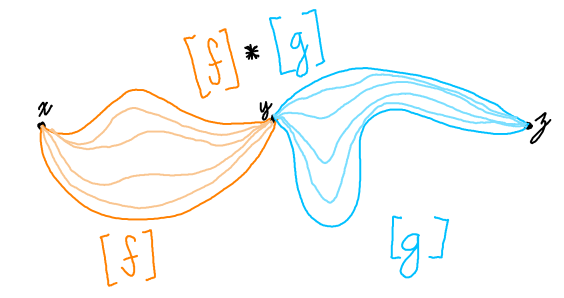
\includegraphics[width=\linewidth]{images/homotopy_class_concat.png}
                \end{center}
            \end{minipage}\\
            \begin{minipage}[c]{\linewidth}
                \begin{center}
                    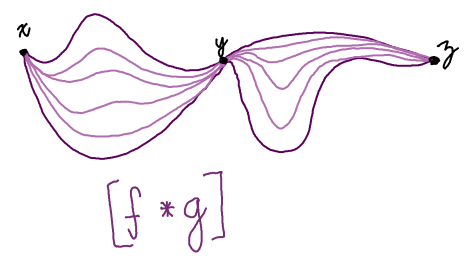
\includegraphics[width=\linewidth]{images/homotopy_class_concat_2.png}
                \end{center}
            \end{minipage}
        \item \underline{Idea of proof of proposition:}\\
            Let,
            \begin{align*}
                F&: I\times I\rightarrow X \text{ be a path homotopy from $f_0$ to $f_1$}\\
                G&: I\times I\rightarrow X \text{ be a path homotopy from $g_0$ to $g_1$}\\
            \end{align*}
            Then we can define,
            \begin{align*}
                H: I\times I \rightarrow X\\
                H(s,y)=\begin{cases}
                    F(2s,t) & \text{if } 0\leq s \leq \frac{1}{2}\\
                    G(2s-1,t) & \text{if } \frac{1}{2}\leq s \leq 1 \\
                \end{cases}\\
            \end{align*}
            Then,
            \begin{align*}
                h_0=H(s,0)&=(f_0*g_0)(s)\\
                h_1=H(s,1)&=(f_1*g_1)(s)\\
                h_t=H(s,t)&=(f_t*g_t)(s) \text{ (some path between $x$ and $z$ )}\\
            \end{align*}
            So, $H$ is a path homotopy from $(f_0*g_0)$ to $(f_1*g_1)$.
    \end{enumerate}

\section{Day 4}
    \subsubsection{Definition of Fundamental Group}
    \begin{itemize}
        \item \underline{Recall:} If,
            \begin{align*}
                f&=\text{path in $X$ from x to y}\\
                g&=\text{path in $X$ from y to z}\\
            \end{align*}
            Then,
            \begin{align*}
                [f]*[g]:=[\text{concatenation $f*g$ of $f$ and $g$}]\\
            \end{align*}
        \item{Properties of $*$:}
            \begin{enumerate}
                \item $*$ is associative, or
                    \begin{align*}
                        [f]*([g]*[h])=([f]*[g])*[h]\\
                    \end{align*}
                    The idea here is that we can adjust the time taken to travel on the path.
                    These two paths are path-homotopic: interpolate between $f*(g*h)$ and
                    $(f*g)*h$ by making f take less and less time and h take more and more time.\\
            \begin{minipage}[c]{\linewidth}
                \begin{center}
                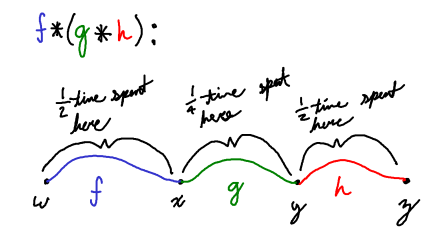
\includegraphics[]{images/association.png}
                \end{center}
            \end{minipage}\\
            \begin{minipage}[c]{\linewidth}
                \begin{center}
                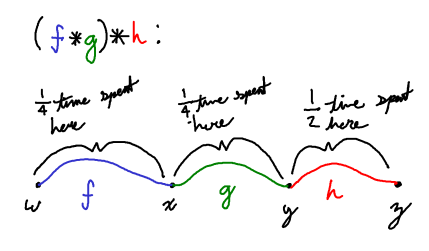
\includegraphics[]{images/association_2.png}
                \end{center}
            \end{minipage}
                \item $*$ has left/right identities.\\
                    Let
                    \begin{align*}
                        e_x&: I\rightarrow X\\
                        e_x(s)&=x,\ \forall\ s\in I, \text{``constant path at $x$''}\\
                    \end{align*}
                    Then, for all paths $f$ from $x$ to $y$, $[f]*[e_y]=[f]$, and
                    $[e_x]*[f]=[f]$. The premise here is that $e_x$ or $e_y$ spend "half
                    the time" sitting at either $x$ or $y$.\\
                    \begin{minipage}[c]{\linewidth}
                        \begin{center}
                            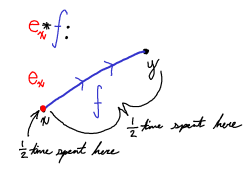
\includegraphics[]{images/path_identity.png}
                        \end{center}
                    \end{minipage}
                    These are path-homotopic: interpolate between $f*e_y$ and $f$ by making
                    $f$ take longer and longer.
                \item $*$ has inverses.\\
                    Let $f$ be a path from $x$ to $y$, and let $\overline{f}$ be the ``reverse'' path,
                    \begin{align*}
                        \overline{f}(s)=f(1-s)\\
                    \end{align*}
                    Then,
                    \begin{align*}
                        [f]*[\overline{f}]&=[e_x]\\
                        [\overline{f}]*[f]&=[e_y]\\
                    \end{align*}\\
                    \begin{minipage}[c]{\linewidth}
                        \begin{center}
                            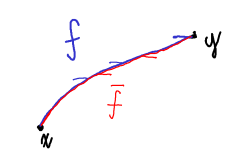
\includegraphics[]{images/path_inverse.png}
                        \end{center}
                    \end{minipage}
                    \underline{Idea:} 
                    The verbal gist of this is that the path takes half the time to travel to its destination, and
                    is concatenated with a path that spends half the time to travel to the origin of the original
                    function.\\
            \end{enumerate}
    \begin{itemize}
        \item
            These are path-homotopic: interpolate between $f*\overline{f}$ and $e_x$ by doing less and less
            of $f$ before turning around.
        \item Let,
            \begin{align*}
                X&=\text{topological space}\\
                x&\in X\\
            \end{align*}
            \begin{definition} A \underline{loop} in $X$ based at $x\in X$ is a path,
            \begin{align*}
                f:I&\rightarrow X\\
                \text{such that}
                &f(0)=f(1)\\
            \end{align*}
            \end{definition}
            \begin{minipage}[c]{\linewidth}
                \begin{center}
                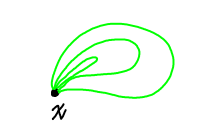
\includegraphics[]{images/loops.png}
                \end{center}
            \end{minipage}
        \item \underline{Observation:} If $f$ and $g$ are any two loops in $X$ based at $x$,
            then $f*g$ is a loop.
    \end{itemize}
            \begin{definition}
                The \underline{fundamental group} of the $X$ with basepoint $x$ is:
                \begin{align*}
                    \pi(X,x)=\{\text{path-homotopy classes of loops in $X$ based at $x$}\}\\
                \end{align*}
                This is a group with the operation $*$\\
            \end{definition}
    \begin{itemize}
        \item $e_x$ and $e_y$ are loops.
        \item $f*\overline{f}$ and $\overline{f}*f$ are also loops.
        \item Good question Katy!
        \item \underline{Note:} The fact that $\pi_1(X,x)$ satisfies the axioms of a group, and follows from the
            properties of $*$ we just checked.\\
            (E.g. the identity element is $[e_x]$)\\
        \item \underline{Question:} What is $\pi_1(\R^2, (0,0))$?\\
            Do you have a guess for $\pi_{1}(S', (1,0))$?\\
            Answer 1: $\pi_1(\R^2, (0,0))\cong \{1\}$\\
            To prove this, it's enough to show that $\pi_1(\R^2, (0,0))$ has just one element,\\
            i.e., any loop in $\R^2$ based at $(0,0)$, is path-homotopic to any other. This is true
            via the straight line homotopy.
            Answer 2: $\pi_1(S', (1,0))\cong \Z$.\\
    \end{itemize}

\section{Day 5}
    \subsubsection{To what extent does $\pi_1$ depend on $x$?}
    \begin{theorem} Let $X$ be a path-connected topological space, and let $x_0,x_1\in X$, then
    $\pi_1(X,x_0)\cong\pi_1(X,x_1)$. This section builds off the worksheet provided in class.
    \begin{enumerate}
        \item \underline{Part 1}: see drawing
        \item \underline{Part 2}: Let $f$ and $g$ be in $\pi_1(X,x_1)$
            \begin{align*}
                \hat{\alpha}([f]*[g])
                &=[\overline{\alpha}] *[f]*[g] *[\alpha]\\
                &=[\overline{\alpha}] *[f] *[\alpha] *[\overline{\alpha}] *[g] *[\alpha]\\
                &=\hat{\alpha}([f])*\hat{\alpha}([g])\\
            \end{align*}
        \item \underline{Part 3}: Let $f \in \pi_1(X,x_1)$
            \begin{align*}
                \hat{\alpha}([f])
                &=[\overline{\alpha}] *[f] *[\alpha]\\
                \hat{\overline{\alpha}}( [\overline{\alpha}] *[f] *[\alpha])
                &=[\alpha] *[\overline{\alpha}] *[f] *[\alpha] *[\overline{\alpha}]\\
                &=[f]\\
            \end{align*}
        \item Therefore this mfer is an isomorphism.
    \end{enumerate}
    \end{theorem}
    \subsubsection{ For which topological spaces $X$ can we actually compute $\pi_1(X,x)$?}
    \begin{definition} A topological space $X$ is \underline{simply-connected} if
    \begin{enumerate}
        \item $X$ is path connected
        \item $\pi_1(X,x)={1}\ \forall x\in X$\\
            (Because $X$ is path connected, we only need to check this for one $x\in X$)
    \end{enumerate}
    \end{definition}
    \begin{itemize}
        \item \underline{Ex:} $\R^2$ is simply connected
        \item \underline{Intuition:} $X$ is simply-connected if any loop in $X$ if any loop in $X$ can
            be ``shrunk down'' to a constant loop.\\
            (for all loops $f$ in $X$ saying $f$ can be ``shrunk down'' means $f\cong_{p}c_x$ where $c_x$ is a constant path)
        \item \underline{Next time:} A convex subset of $\R^n$ is simply connected.
    \end{itemize}

\subsection{Day 6}
    \begin{enumerate}
        \item \underline{Goal:} Prove that $\pi_{1}(S^1, x)\cong \Z$
        \item \underline{Idea:} $S^1$ can be built by ``wrapping $\R$ around itself''.\\:
            %include spirally drawing of Real numbers mapping to S^1%
            Concretely, this is
            \begin{align*}
                p&: \R \rightarrow S^1\\
                p(x)&=(\cos(2\pi x), \sin(2\pi x))\\
            \end{align*}
            We'll try to ``unwrap'' loops in $S^1$ to get paths in $\R$
        \item
            The above map $p$ is an example of a ``covering map''. The ultimate goal of today is to understand
            what it means to be a covering map, before we get to the definition of it.\\
        \item \underline{Questions:} Let the following be so,
            \begin{align*}
                u_1&=\{(x,y)\in S^1| y>0\}\\
                u_2&=\{(x,y)\in S^1| x>0,\ y<0\}\\
            \end{align*}
            Include the drawings from class, really get sick wit it.
        \item \underline{Observation:} For any particular $n\in \Z$, the piece,
            \begin{align*}
                (n, n+\frac{1}{2})\cong u_1\\
            \end{align*}
            The homeomorphism in Dr. Clader's mind is,
            \begin{align*}
                \phi&: (n,n+\frac{1}{2})\rightarrow u_1\\
                \phi(x)&=(\cos(2\pi x), \sin(2\pi x))\\
                \text{i.e. } \phi&=p_{|(n,n+\frac{1}{2})}\\
            \end{align*}
            The inverse of $\phi$ is,
            \begin{align*}
                \phi^{-1}: u_1&\rightarrow(n,n+\frac{1}{2})\\
                \phi^{-1}&=\frac{\cos^{-1} (x)}{2\pi}+n\\
                (\text{Recall: by }&\text{definition}\ \cos^{-1}(x)\in[0,\pi])\\
            \end{align*}
            Similarly, for $u_2$ for any particular $n\in \Z$, $(n-\frac{1}{4}, n)\cong u_2$.
        \item \underline{Definition:} Let $p:E \rightarrow B$ be a function between two topological spaces. We say
            $p$ is a \underline{covering map} if $p$ is,
            \begin{enumerate}
                \item $p$ is continuous and surjective
                \item $\forall b\in B$ there exists a neighborhood $u$ of b such that,
                    \begin{align*}
                        p^{-1}(u)=\cup_{\alpha}v_{\alpha}\\
                    \end{align*}
                    where $v_\alpha\subseteq E$ are open, disjoint and,
                    \begin{align*}
                        p_{|v_{\alpha}}:v_{\alpha}\rightarrow u\\
                    \end{align*}
                    is a homeomorphism for every $\alpha$. Note that these open subsets with this property are called
                    \underline{evenly covered}\\
                    %see the classroom drawing, think about pancakes%
                    Note that $b$ is one particular point or neighborhood, but there should be a neighborhood for every single
                    point in $B$ where all of this junk holds reasonably truish.
            \end{enumerate}
        \item \underline{Ex:}
            \begin{align*}
                p: \R \rightarrow S^1\\
                p(x)=(\cos(2\pi x), \sin(2\pi x))\\
            \end{align*}
            $p$ is a covering map. We just showed that $u_1$ is evenly covered:
            \begin{align*}
                p^{-1}(u_1)=\cup_{n\in \Z}(n,n+\frac{1}{2})\\
            \end{align*}
            Note that in this case the $(n, n+\frac{1}{2})$ are the $v_\alpha$ from the definition of
            covering maps. $u_2$ is also evenly covered, but, $U=S^{1}$ is not evenly covered because,
            $p^{-1}(S^{1})=\R$, and the only way to write $\R$ as a uniion of disjoint open sets $v_\alpha$,
            is to take $v_\alpha=\R$, but $\R \ncong S^1$
        \item \underline{Ex:}
            \begin{align*}
                B=\text{any space}\\
                E=B\times \{1,2,...,n\}=\text{n discrete copies of $B$}\\
            \end{align*}
            Where $\{1,2,...,n\}$ is equipped with the discrete topology.
    \end{enumerate}

\documentclass[../notes.tex]{subfiles}
\begin{document}
\section{Day 7}
    \subsubsection{Guest lecturer: Mattias ``your regular lecturer is more qualified for this'' Beck}
    \begin{itemize}
        \item Recalling the definition of an evenly covered set. New notation was introduced, but
            \LaTeX is behind the times.
            Let $E$ and $B$ be topological spaces
            %\hookrightarrow for injectivity
            \begin{align*}
                \phi&:E \twoheadrightarrow B\\
                \forall b \in B,&\ \exists u\ \text{a neighborhood of b}: p^{-1}(u)=\cup_{\alpha}v_\alpha\\
                p_{|v_{\alpha}}&: v_{\alpha}\rightarrow u\\
            \end{align*}
        \item \underline{Fun notation facts:}\\
            $\twoheadrightarrow$ indicates a surjective function\\
            $\hookrightarrow$ indicates an injective function\\
            Combining the two gives you a bijective function, but that symbol doesn't exist
            in latex apparently.
        \item \underline{Example covering:}
            \begin{align*}
                E&=\R\\
                \phi(x)&=(\cos(2\pi x), \sin(2\pi x))\\
                B&=S^{1}\\
            \end{align*}
    \end{itemize}
            \begin{definition} Given a covering map from topological
                spaces $E$ to $B$
                \begin{align*}
                    p: E\rightarrow B\\
                \end{align*}
                    a path in our topological space B,
                \begin{align*}
                    f: I \rightarrow B\\
                \end{align*}
                A \underline{lift} of $f$ is a path, $\tilde{f}: I\rightarrow E$, such that
                $f=p\circ \tilde{f}$
            \end{definition}
    \begin{itemize}
        \item 
            This is theoretically a theorem.\\
            Given covering map $p:E\rightarrow B$, $p(e)=b$,
            $f:I \rightarrow B$ path beginning at b, then there does not exist a left $\tilde{f}$,
            of $f$ beginning at $e$ Read Lemma 54.1 Munkres. (?!?!?)
    \end{itemize}
    \begin{theorem}
        Let the following be so,
        \begin{align*}
            E& \text{ be a topological space}\\
            B& \text{ be a topological space}\\
            p&:E \rightarrow B \text{ a covering map}\\
            f&:I \rightarrow B \text{ path beginning at $b$ }\\
            e &\in E,\ s.t.\ p(e)=b\\
        \end{align*}
        Then there exists a unique path, $\tilde{f}$ in $E$ such that $p\circ \tilde{f}=f$, and
        $\tilde{f}(0)=e$
    \end{theorem}
\end{document}
\section{Day 8}
    \begin{enumerate}
        \item \underline{Guest Lecturer:} Matthias ``you can have a hint, but you can't quote me on it'' Beck
        \item ???????
    \end{enumerate}

\documentclass[../notes.tex]{subfiles}
\begin{document}
\section{Day 9}
    \subsubsection{Guest Lecturers: Anastasia the Assassin, Deadly David, and Killa Katy}
    \begin{itemize}
        \item Let $p$ be a covering map.
            \begin{align*}
                p: E\rightarrow B\\
            \end{align*}
            Let, $e\in E$, $b\in B$, such that $p(e)=b$.\\
            Summary of what we know about this situation,
            \begin{enumerate}
                \item Any path $f$ in $B$, beginning at $b$ has a unique lift $\tilde{f}$ to a path in $E$ beginning at $e$.
                \item If $f$ and $g$ are two paths in $B$, beginning at $b$, such that $f\cong_{p}g$, then
                    $\tilde{f}\cong_{p}\tilde{g}$
                \item If $f$ is a loop in $B$ based at $b$, then $\tilde{f}\in p^{-1}(b)$
            \end{enumerate}
    \end{itemize}
\end{document}
\section{Day 10}
    \subsubsection{$\pi_1(S^1)$, continued:}
    \begin{itemize}
        \item \underline{Recap:}
            \begin{align*}
                p&: \R \rightarrow S^{1}\\
                p(x)&=(\cos(2\pi x), \sin(2\pi x))\\
            \end{align*}
            Then there exists a function,
            \begin{align*}
                \phi &: \pi_1(S^{1}, b)\rightarrow p^{-1}(b)\\
                \phi([f])&=\tilde{f}(1)\\
            \end{align*}
            Where $\tilde{f}$ is the lift of $f$ to $\R$ starting at $0$.\\
            E.g.,(draw that spiraleboye)
            \begin{align*}
                \phi&([\text{loop once counterclockwise}])=1\\
                \phi&([\text{loop twice counterclockwise}])=2\\
                \phi&([\text{loop once clockwise}])=-1\\
            \end{align*}
            The fact that there exists a unique lift, $\tilde{f}$ of any $f$ is a feature
            of covering maps.\\
            In fact,
            \begin{align*}
                p^{-1}(b)=\Z\\
            \end{align*}
            and,\\
        \item \underline{Claim:} $\phi: \pi_1(S^1, b)\rightarrow \Z$ is a bijection.
            \begin{proof}
                \begin{enumerate}
                    \item \underline{Surjective:} Given $c\in\Z$, choose a path, $\alpha: I \rightarrow \R$, from
                        $0$ to $c$ in $\R$. Then let, $f: I \rightarrow S^1$ be $f=p\circ \alpha$\\
                        Then f is a loop in $S^1$ based at $b=(1,0)$ because
                        \begin{align*}
                            f(0)=p(\alpha(0))=p(0)=(1,0)\\
                            f(1)=p(\alpha(1))=p(c)=(1,0)\\
                        \end{align*}
                        And, $\tilde{f}=\alpha$ because $p\circ \tilde{f}=p\circ \alpha = f$. Thus,
                        \begin{align*}
                            \phi([f])=\tilde{f}(1)=\alpha(1)=c\\
                        \end{align*}
                    \item \underline{Injective:} Suppose,
                        \begin{align*}
                            \phi([f])=\phi([g])\\
                            \implies \tilde{f}(1)=\tilde{g}(1)\\
                        \end{align*}
                        Then, $\tilde{f}$ and $\tilde{g}$ are two paths in $\R$, that both start at 0
                        and both end at the same point.\\
                        $\Rightarrow$ (courtesy of homework 2) $\tilde{f}\cong_{p}\tilde{g}$ (because $\R$ is simply
                        connected)\\
                        $\Rightarrow$ $p\circ H$ is a path homotopy from $p\circ \tilde{f}$ to $p\circ \tilde{g}$.\\
                        $\Rightarrow f\cong_{p}g$\\
                        $\Rightarrow [f]=[g]\in \pi_1(S^1, b)$\\
                \end{enumerate}
            \end{proof}
        \item \underline{Claim:} $\phi$ is a group homomorphism ( thus, an isomorphism ).\\
            \begin{proof}
                Let $[f], [g]\in \pi \pi_1(S^1,b)$, we want to show that,
                $\phi([f]*[g])=\phi([f])+\phi([g])$\\
                By definition,
                \begin{align*}
                    \phi([f]*[g])=\phi([f*g])=\tilde{f*g(1)}\\
                \end{align*}
                What is $\tilde{f*g}$? By definition $\tilde{f*g}$ is the lift of $f*g$
                starting at $0$ and,
                \begin{align*}
                    \tilde{f}=\text{lift of $f$ starting at 0 ending at some $n$}\\
                    \tilde{g}=\text{lift of $g$ starting at 0 ending at some $m$}\\
                \end{align*}
                %Note some drawing.
                So, $\tilde{f}*\tilde{g}$ doesn't make sense, but let:
                \begin{align*}
                    \tilde{g}^{\prime}&=\text{``shift $\tilde{g}$ by n ''}\\
                    \text{i.e., }\tilde{g}^{'}&=g(s)+n\\
                \end{align*}
                Sow notice that $\tilde{f}*\tilde{g}^{'}$ now makes sense, and $\tilde{g}^{'}$ is a
                lift of $g$, because:
                \begin{align*}
                    (p\circ\tilde{g}^{'})(s)&=p(\tilde{g}(s))\\
                    &=p(\tilde{g}(s)+n)\\
                    &=p(\tilde{g}(s))\\
                \end{align*}
                    because $p(x+n)=p(x) $\forall n\in\Z$
                \begin{align*}
                    &=(p\circ\tilde{g})(s)\\
                    &=g(s)\\
                \end{align*}
                Thus, $\tilde{f}*\tilde{g}^{'}$ is a lift of $f*g$ starting at $0$\\
                \begin{align*}
                    \implies \tilde{f}*\tilde{g}&=\tilde{f*g}\\
                    \tilde{f*g}(1)&=\tilde{f}*\tilde{g}\\
                    &=\text{endpoint of $\tilde{g}^{\prime}$}\\
                    &=\tilde{g}(1)+n\\
                    &=m+n\\
                \end{align*}
                This shows that
                \begin{align*}
                    \phi([f]*[g])&=m+n\\
                    &=\tilde{f}(1)+\tilde{g}(1)\\
                    &=\phi([f])+\phi([g])\\
                \end{align*}
            \end{proof}
        \item \underline{We want:}
            \begin{align*}
                X\cong Y\implies \pi_1(X,x)\cong\pi_1(Y,y)\\
                \text{(X is homeomorphic to Y)}\\
            \end{align*}
            The big tool we'll use to do that is the tool from the second homework
            about maps between spaces being homomorphisms. That's for next time!
    \end{itemize}

\section{Day 11}
    \subsubsection{Examining the group structure of $*$ functions}
    \begin{enumerate}
        \item Note that this Friday, office hours will be at 3-4pm.
        \item \underline{We want:} If $X\cong Y$, then $\pi_1(X,x)\cong \pi_1(Y,y)$,
            or that, if two spaces are homeomorphic, then their fundamental groups are isomorphic. We
            will explore the tools used to show this in this lecture. From homework 2, we get the following
            definition
        \item 
            \begin{definition}
                Let $\varphi: X\rightarrow Y$, be a continuous
                map, then the \underline{homomorphism induced by $\varphi$} is:
                \begin{align*}
                    \varphi_{*}: \pi_1(X,x)\rightarrow \pi_1(Y,y)\\
                    \varphi_{*}([f])=[\varphi\circ f]\\
                \end{align*}
                See the picture of the picture drawn on the board, make a drawyboye.
            \item \underline{Lemma:} (this is referred to lemma 1)If
                \begin{align*}
                    X\rightarrow^{\varphi}Y\rightarrow^{\psi}Z\\
                \end{align*}
                Where $\varphi$ and $\psi$ are both continuous, then,
                \begin{align*}
                    (\psi \circ \varphi)_{*}=\psi \circ_{*} \varphi_{*}\\
                \end{align*}
                Additionally, (This is referred to as lemma 2)
                \begin{align*}
                    {id}_{*}=id\\
                \end{align*}
                (or that given the $id: X\rightarrow Y$, the induced homomorphism,
                $\pi_{1}(X,x)\rightarrow \pi_{1}(Y,y)$ is the identity)
            \end{definition}
        \item \begin{proof}
                    Firstly, Both sides are homomorphisms
                        \begin{align*}
                            \pi_1(X,x)\rightarrow\pi_1(Z,(\psi\circ\varphi)(x))\\
                        \end{align*}
                    Given any $[f]\in\pi_1(X,x)$:
                        \begin{align*}
                            (\psi\circ\varphi)_{*}([f])=[(\psi\circ\varphi)\circ f]\\
                            =[\psi\circ(\varphi\circ f)]\\
                            =\psi_{*}[\varphi\circ f]\\
                            =\psi_{*}(\varphi_{*}(f))\\
                            =(\psi_{*}\circ\varphi_{*})([f])\\
                        \end{align*}
                    Given any $[f]\in\pi_1(X,x)$:
                        \begin{align*}
                            id_{*}([f])=[id\circ f]\\
                            =[f]\\
                        \end{align*}
        \end{proof}
        \item 
            \begin{theorem} if $\varphi: X\rightarrow Y$ is a homeomorphism,
            then $\varphi_{*}: \pi_{1}(X,x)\rightarrow\pi_{1}(Y,y)$ is an isomorphism.
            \end{theorem}
                \begin{proof}
                    We already know that $\varphi_{*}$ is a homomorphism, to prove that it's
                    a bijection, we'll find an inverse to $\varphi_{*}$. Claim that,
                    \begin{align*}
                        (\varphi)_{*}:\pi_1(Y,\varphi(x))\rightarrow\pi_1(X,x)\\
                    \end{align*}
                    is the inverse to $\varphi_{*}$.\\
                    (Note that this is doable, because $\varphi$ is a homeomorphism, $\varphi^{-1}:Y\rightarrow X$ exists, and is continuous)\\
                    To check this:
                    \begin{align*}
                        \varphi_{*}\circ (\varphi^{-1})\\
                        =(\varphi\circ\varphi^{-1}),\ \text{by lemma 1 shown today}\\
                        =id_{*},\ \text{by definition of $\varphi^{-1}$ (identity on y)}\\
                        =id,\ \text{by lemma 2 shown today (identity on x)}\\
                        (\varphi^{-1})_{*}\circ\varphi_{*}=(\varphi^{-1}\circ\varphi)_{*}=id_{*}=id\\
                    \end{align*}
                    This by definition means $\varphi_{*}$ and $(\varphi^{-1})_{*}$ are inverse functions.
                    Additionally, this small red box has made it onto the board, for clarification.
                    \begin{align*}
                        id_x: X \rightarrow Y\\
                        id_{\pi_1(X,x)}:\pi_1(X,x)\rightarrow\pi_1(X,x)\\
                        \text{Lemma: }(id_{x})_{*}id_{\pi_1(X,x)}\\
                    \end{align*}
                \end{proof}
        \item
            This ends up proving that,
            \begin{align*}
                X\cong Y\implies\pi_1(X,x)\cong\pi_1(Y,\varphi(x))\\
            \end{align*}
            But, non-homeomorphic spaces \underline{can} have isomorphic $\pi_{1}$\\
            \underline{Ex:}
            \begin{align*}
                X=.\\
                Y=\R^2\\
            \end{align*}
            These are not homeomorphic, clearly X is compact and Y isn't, but their fundamental groups are
            isomorphic, since the fundamental group of $X$ is just $\{1\}$, and clearly this is also true
            about $\R^2$
        \item So, given $X$ and $Y$, how can we tell if $\pi_1(X)\cong\pi_1(Y)$?
    \end{enumerate}
        \subsubsection{Homotopy of Maps:}}
            \begin{definition} Let $f: X\rightarrow Y$ and $g: X\rightarrow Y$ be continuous functions.
            Then a \underline{homotopy} from $f$ to $g$ is a continuous function,
            \begin{align*}
                H: X\times I\rightarrow Y\\
            \end{align*}
            such that,
            \begin{align*}
                H(x,0)=f(x),\ \forall x\in X\\
                H(x,1)=f(x),\ \forall x\in X\\
            \end{align*}
            Our goal is to make remark about the lower star versions of these maps, given their being homotopic.
            \end{definition}

\section{Day 12}
    \begin{enumerate}
        \item \underline{Homotopy of maps:}
            \underline{Definition:} Let $f: X\rightarrow Y$ be a continuous function.
            A \underline{homotopy} from $f$ to $g$ is a continuous function,
            \begin{align*}
                H:X\times I \rightarrow Y\\
                \text{such that}\\
                H(x,0)=f\\
                H(x,0)=g\\
            \end{align*}
            We'll often write,
            \begin{align*}
                h_t:X \rightarrow Y\\
                h_t(x)=H(x,t)\\
            \end{align*}
            Then there's one $h_t$ for each $t\in I$ and,
            \begin{align*}
                h_0=f\\
                h_1=g\\
                h_t=\text{``A function interpolating between $f$ and $g$''}\\
            \end{align*}
        \item \underline{Terminology/Notation:} If there exists a homotopy from
            $f$ to $g$, we'll say that \underline{$f$ is homotopic to $g$} and write
            $f\cong g$.\\
        \item \underline{Ex:}
            \begin{align*}
                f: S^{1}\rightarrow \R^2\\
                g: S^{1}\rightarrow \R^2\\
                f(x,y)=(x,y)\\
                g(x,y)=(0,0)\\
            \end{align*}
            Then $f\cong g$. A homotopy from $f$ to $g$ is,
            \begin{align*}
                H: S^{1}\times I \rightarrow \R^2\\
                H((x,y),t)=((1-t)x,(1-t)y)\\
            \end{align*}
            Do the drawing from the board.
        \item \underline{Ex:}
            \begin{align*}
                f:\R \rightarrow \R\\
                g:\R \rightarrow \R\\
                f(x)=x\\
                g(x)=x+2\\
            \end{align*}
            Then $f\cong g$. A homotopy from $f$ to $g$ is:
            \begin{align*}
                H:\R \times I \rightarrow \R\\
                H(x,t)=x+2t\\
            \end{align*}
            Refer again to the picture from the board.
        \item \underline{Questions:}
            \begin{enumerate}
                \item
                    \begin{align*}
                        f: \R \rightarrow \R^2\\
                        g: \R \rightarrow \R^2\\
                        f(x)=(x,0)\\
                        g(x)=(x,e^x)\\
                    \end{align*}
                \item
                    \begin{align*}
                        f: \R^2\setminus{(0,0)} \rightarrow \R^2\setminus{(0,0)}\\
                        g: \R^2\setminus{(0,0)} \rightarrow \R^2\setminus{(0,0)}\\
                        f(x)=(x,y)\\
                        g(x)=(\frac{x}{\sqrt{x^2+y^2}},\frac{y}{\sqrt{x^2+y^2}})\\
                    \end{align*}
                    \begin{align*}
                        f: \R \rightarrow \R^2\\
                        g: \R \rightarrow \R^2\\
                        f(x)=(x,0)\\
                        g(x)=(x,e^x)\\
                    \end{align*}
                    Just use the straight line homotopy it's not hard.
            \end{enumerate}
            Maybe include the drawings?
        \item \underline{Definition:} Let $f:X\rightarrow Y$ and $g: X\rightarrow Y$ be continuous,
            and let $x_0 \in X$ be such that $f(x_0)=g(x_0)=y_0$. Then a
            \underline{homotopy from $f$ to $g$ relative to $x_0$} is a homotopy $H:X\times I \rightarrow Y$
            from $f$ to $g$ such that $h_t(x_0)=y_0,\ \forall t$.\\
            (``$x_0$ doesn't move during the homotopy'')
        \item \underline{Ex:} in the second part of the questions from today, $H$ was a homotopy relative to $(1,0)$, or
            to any other point on the unit circle.
        \item \underline{Ex:}
            \begin{align*}
                X=\{(x,y)\in \R^2 | x^2+y^2\leq 1\}\\
            \end{align*}
            (it's the 2 norm ball)
            \begin{align*}
                f: X\rightarrow X\\
                g: X\rightarrow X\\
            \end{align*}
            Then,
            \begin{align*}
                H: X\times I \rightarrow X\\
                H((x,y),t)=(1-t)x, (1-t)y)\\
            \end{align*}
            is a homotopy relative to $(0,0)$.
        \item \underline{Theorem:} If $f:X\rightarrow Y$ and $g:X\rightarrow Y$ are
            homotopic relative to $x_0$, then:
                \begin{align*}
                    f_{*}:\pi_1(X,x_0)\rightarrow \pi_1(Y,y_0)\\
                    g_{*}:\pi_1(X,x_0)\rightarrow \pi_1(Y,y_0)\\
                \end{align*}
                are the same homomorphism.
    \end{enumerate}

\end{document}

\section{Notes}


